% ============================================================
%  News Credibility Monitor — Milestone 1 Report
%  Intelligent News Credibility Analysis using Traditional ML
% ============================================================

\documentclass[12pt, a4paper]{article}

% ---- Packages ----
\usepackage[utf8]{inputenc}
\usepackage[T1]{fontenc}
\usepackage{lmodern}
\usepackage[margin=1in]{geometry}
\usepackage{graphicx}
\usepackage{booktabs}
\usepackage{hyperref}
\usepackage{amsmath}
\usepackage{float}
\usepackage{enumitem}
\usepackage{listings}
\usepackage{xcolor}
\usepackage{caption}
\usepackage{subcaption}
\usepackage{fancyhdr}
\usepackage{setspace}

% ---- Page Style ----
\pagestyle{fancy}
\fancyhf{}
\rhead{Milestone 1 — Mid-Sem Capstone}
\lhead{News Credibility Monitor}
\rfoot{Page \thepage}

% ---- Code Listing Style ----
\lstset{
    language=Python,
    basicstyle=\ttfamily\small,
    keywordstyle=\color{blue}\bfseries,
    commentstyle=\color{gray}\itshape,
    stringstyle=\color{red},
    frame=single,
    breaklines=true,
    numbers=left,
    numberstyle=\tiny\color{gray},
    backgroundcolor=\color{gray!5},
}

% ---- Hyperlinks ----
\hypersetup{
    colorlinks=true,
    linkcolor=blue,
    citecolor=blue,
    urlcolor=blue,
}

% ---- Title ----
\title{
    \vspace{-1cm}
    \textbf{Intelligent News Credibility Analysis} \\[0.3cm]
    \large Milestone 1: Traditional Machine Learning Approach \\[0.2cm]
    \large GenAI Capstone Project — Mid-Semester Evaluation
}
\author{
    Aryan Kinha
    Divyanshu Singh
    Jatin Kumar Singh
    Jatin Verma\\
    Rishihood University, Newton School of Technology \\
}
\date{March 2026}

\begin{document}

\maketitle
\thispagestyle{fancy}

% ============================================================
\begin{abstract}
Misinformation in digital news poses a significant threat to public discourse and democratic processes. This project presents an end-to-end machine learning system for binary classification of news articles as \textit{Real} or \textit{Fake}. We employ a Natural Language Processing (NLP) pipeline consisting of text preprocessing, TF-IDF vectorization with bigram features, and Logistic Regression with class-balanced weighting. Trained and evaluated on the ISOT Fake News Dataset (44,898 articles), the system achieves \textbf{98.88\% accuracy}, \textbf{98.88\% weighted F1-score}, and is deployed as an interactive web application via Streamlit Community Cloud. The modular codebase follows a production-ready architecture with separated concerns for data ingestion, feature engineering, model training, evaluation, and inference.
\end{abstract}

\tableofcontents
\newpage

% ============================================================
\section{Introduction}

\subsection{Problem Statement}
The proliferation of fake news on social media and digital platforms has become a critical societal challenge. Manual fact-checking is inherently unscalable, creating a need for automated systems capable of assessing news credibility at scale. This project addresses the binary classification problem: given a news article, determine whether it is \textit{Real} (credible) or \textit{Fake} (fabricated/unreliable).

\subsection{Objectives}
\begin{enumerate}[label=\arabic*.]
    \item Design and implement a modular ML pipeline for fake news detection.
    \item Achieve high classification performance using traditional ML techniques (no LLMs).
    \item Deploy the trained model as an accessible web application.
    \item Document design choices and justify each architectural decision.
\end{enumerate}

\subsection{Scope \& Constraints}
\begin{itemize}
    \item \textbf{Milestone 1 Constraint:} Only traditional ML methods are permitted — no Large Language Models (LLMs) or Agentic AI.
    \item \textbf{Domain:} The model is trained on US political and world news articles (2016–2018).
    \item \textbf{Deliverables:} Source code, Streamlit demo, this report, and a 5-minute project video.
\end{itemize}

% ============================================================
\section{Dataset}

\subsection{ISOT Fake News Dataset}
We use the ISOT Fake News Dataset\footnote{\url{https://onlineacademiccommunity.uvic.ca/isot/2022/11/27/fake-news-detection-datasets/}}, a widely-used benchmark for fake news detection research.

\begin{table}[H]
\centering
\caption{Dataset Composition}
\begin{tabular}{@{}lrrr@{}}
\toprule
\textbf{Class} & \textbf{Articles} & \textbf{Percentage} & \textbf{Source} \\
\midrule
Real & 21,417 & 47.7\% & Reuters \\
Fake & 23,481 & 52.3\% & Politifact/Wikipedia-flagged sources \\
\midrule
\textbf{Total} & \textbf{44,898} & 100\% & — \\
\bottomrule
\end{tabular}
\end{table}

\subsection{Data Splitting}
An 80/20 stratified train-test split with \texttt{random\_state=42} ensures reproducibility:

\begin{table}[H]
\centering
\caption{Train-Test Split}
\begin{tabular}{@{}lrr@{}}
\toprule
\textbf{Split} & \textbf{Samples} & \textbf{Percentage} \\
\midrule
Training Set & 35,918 & 80\% \\
Test Set & 8,980 & 20\% \\
\bottomrule
\end{tabular}
\end{table}

\subsection{Feature Construction}
Both the \texttt{title} and \texttt{text} columns are concatenated to form a single input feature: $\text{input} = \text{title} \oplus \text{text}$. This provides richer semantic context than using article text alone, as headlines often contain distinctive stylistic cues.

% ============================================================
\section{Methodology}

\subsection{System Architecture}
The system follows a modular pipeline architecture with clear separation of concerns:

\begin{figure}[H]
\centering
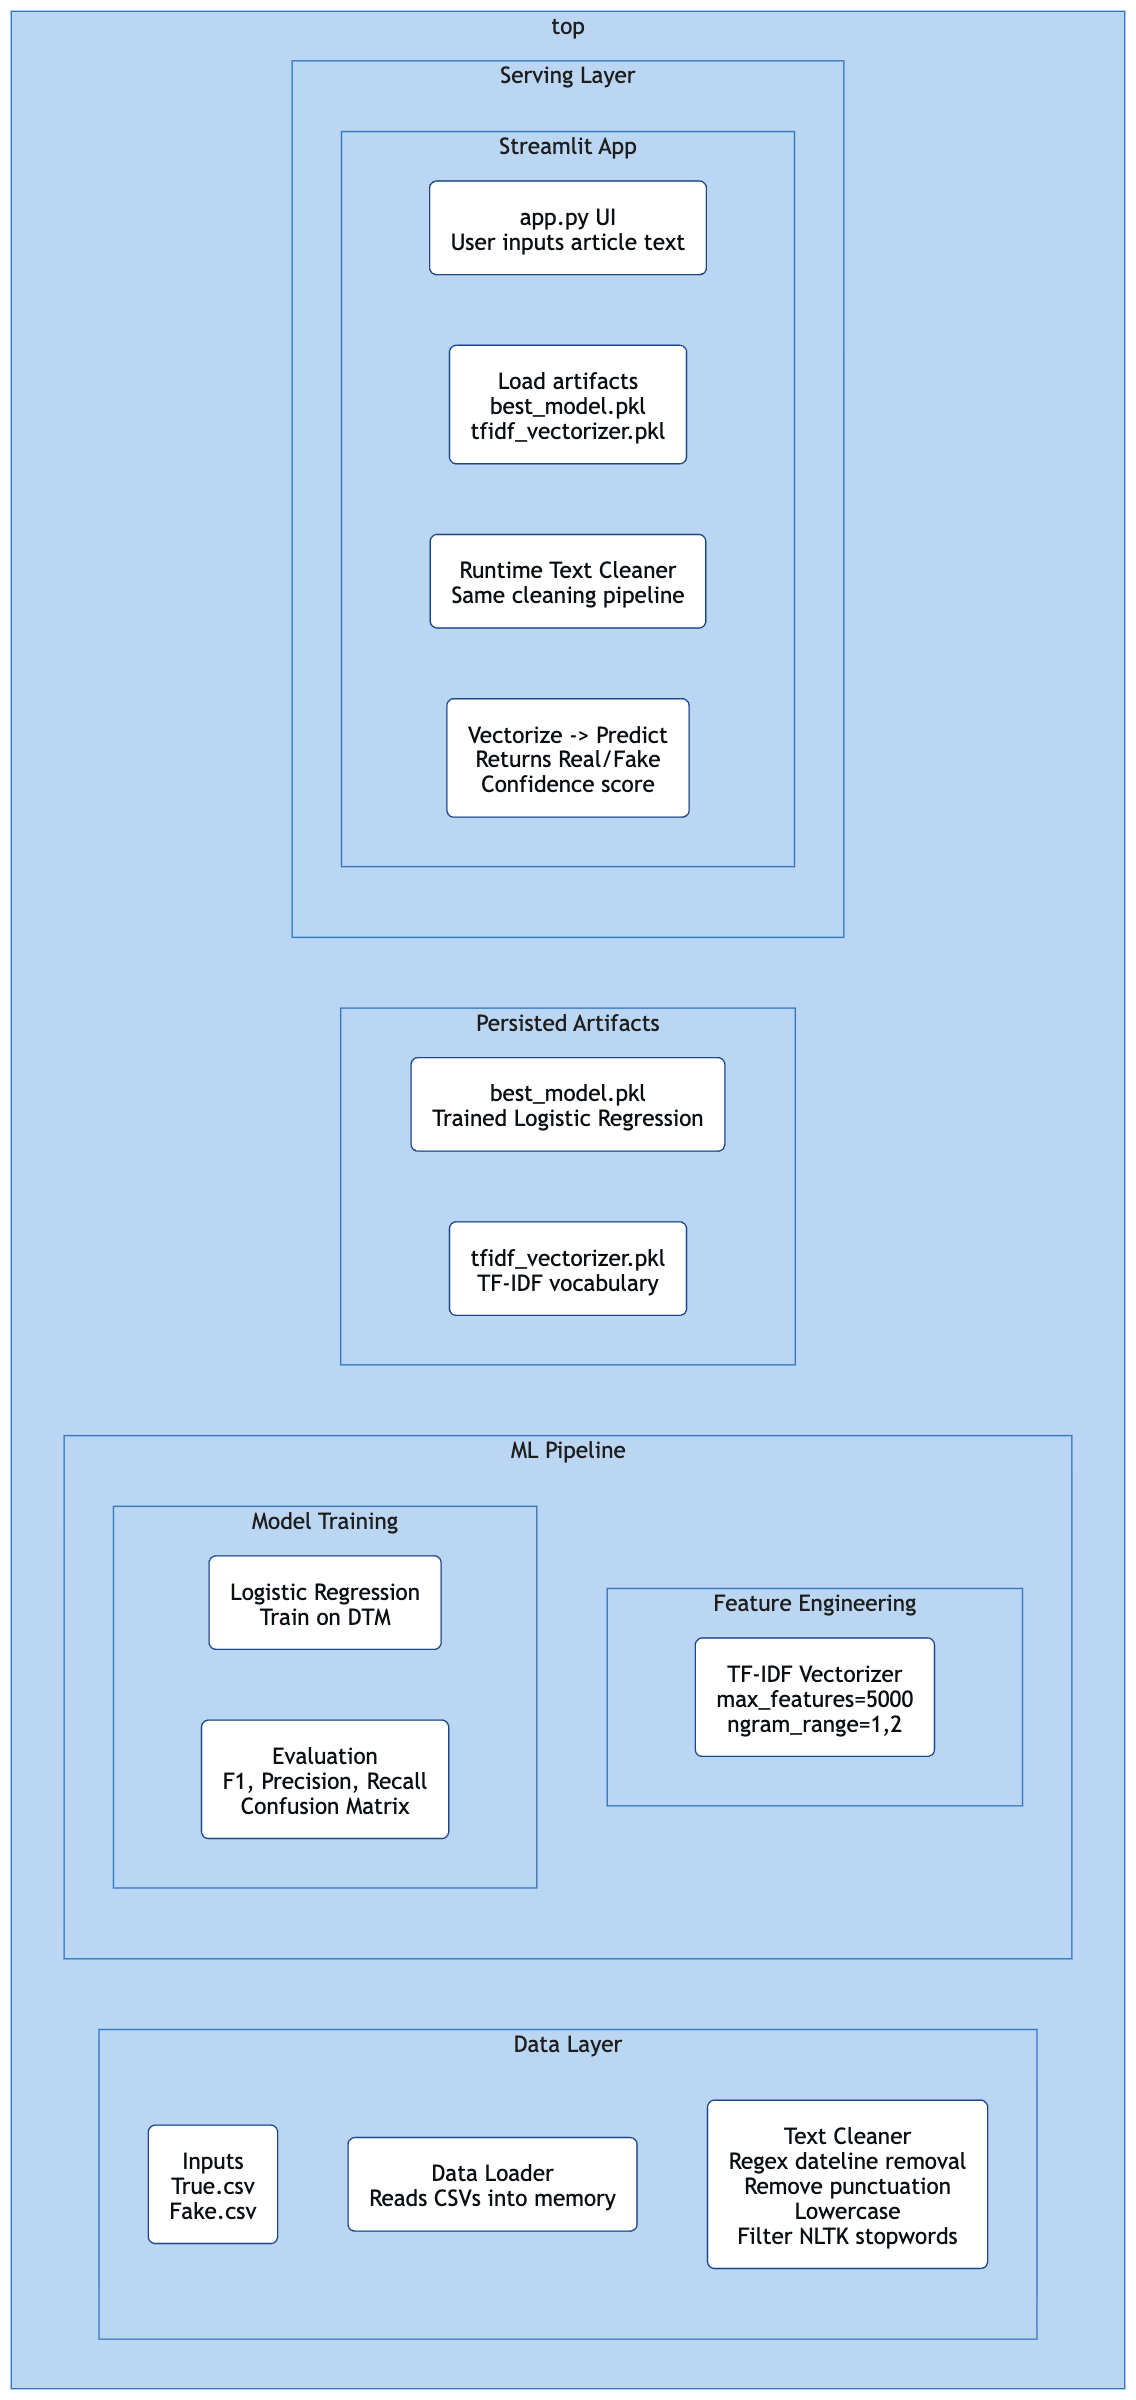
\includegraphics[width=0.85\textwidth]{../docs/system_design.png}
\caption{End-to-end system architecture from data ingestion to deployment.}
\label{fig:architecture}
\end{figure}

The pipeline is organized into five distinct modules:
\begin{enumerate}
    \item \textbf{Data Ingestion} (\texttt{src/data/load\_data.py}) — Loads, labels, merges, and shuffles raw CSVs.
    \item \textbf{Text Preprocessing} (\texttt{src/utils/text\_cleaner.py}) — Cleans and normalizes raw text.
    \item \textbf{Feature Engineering} (\texttt{src/features/build\_features.py}) — TF-IDF vectorization.
    \item \textbf{Model Training} (\texttt{src/models/train.py}) — Logistic Regression training.
    \item \textbf{Evaluation} (\texttt{src/models/evaluate.py}) — Metrics computation and export.
\end{enumerate}

\subsection{Text Preprocessing Pipeline}
The preprocessing pipeline in \texttt{text\_cleaner.py} applies four transformations sequentially:

\begin{enumerate}
    \item \textbf{Dateline Stripping:} Removes publisher prefixes (e.g., \texttt{"WASHINGTON (Reuters) -"}) to prevent source-name leakage into the feature space.
    \item \textbf{Lowercasing:} Converts all characters to lowercase for case-invariant matching.
    \item \textbf{Special Character Removal:} Strips non-alphabetic characters via the regex pattern \texttt{[{\textasciicircum}a-zA-Z\textbackslash s]}.
    \item \textbf{Stopword Removal:} Filters 179 English stopwords from NLTK's corpus.
\end{enumerate}

\textbf{Design Decision — Dateline Stripping:} Without this step, the model could trivially learn that articles containing \texttt{"(Reuters)"} are real, leading to inflated accuracy that would not generalize to articles from other sources.

\subsection{Feature Engineering: TF-IDF Vectorization}

We use Term Frequency–Inverse Document Frequency (TF-IDF) to convert cleaned text into numerical feature vectors:

\begin{equation}
\text{TF-IDF}(t, d) = \text{TF}(t, d) \times \log\left(\frac{N}{\text{DF}(t)}\right)
\end{equation}

where $t$ is a term, $d$ is a document, $N$ is the total number of documents, and $\text{DF}(t)$ is the number of documents containing $t$.

\textbf{Configuration:}
\begin{itemize}
    \item \texttt{max\_features = 10,000} — Retains the top 10,000 most informative terms.
    \item \texttt{ngram\_range = (1, 2)} — Captures both unigrams and bigrams (e.g., ``breaking news'', ``sources say'').
\end{itemize}

\textbf{Justification for 10,000 features:} Empirical experiments in Notebook 03 compared 5,000 vs.\ 10,000 features. The larger vocabulary marginally improves recall on the Fake class by capturing less-frequent but discriminative bigrams, with negligible impact on training time due to the sparsity of TF-IDF matrices.

\subsection{Model: Logistic Regression}

\textbf{Why Logistic Regression?}
\begin{enumerate}
    \item \textbf{Interpretability:} Feature coefficients directly reveal which words/phrases are most indicative of fake or real news, enabling model transparency.
    \item \textbf{Strong Baseline:} Logistic Regression consistently achieves competitive performance on text classification tasks with high-dimensional sparse features~\cite{joachims1998text}.
    \item \textbf{Computational Efficiency:} Training completes in seconds, enabling rapid iteration. Inference is sub-millisecond, suitable for real-time deployment.
    \item \textbf{Probabilistic Output:} The sigmoid function naturally produces calibrated probability scores, used as confidence indicators in the Streamlit app.
\end{enumerate}

\textbf{Hyperparameters:}
\begin{table}[H]
\centering
\caption{Logistic Regression Hyperparameters}
\begin{tabular}{@{}llp{7cm}@{}}
\toprule
\textbf{Parameter} & \textbf{Value} & \textbf{Justification} \\
\midrule
\texttt{solver} & \texttt{lbfgs} & Limited-memory BFGS; efficient for L2-regularized problems with large feature spaces. \\
\texttt{max\_iter} & 1000 & Ensures convergence on high-dimensional TF-IDF features. \\
\texttt{class\_weight} & \texttt{balanced} & Automatically adjusts weights inversely proportional to class frequencies, correcting the 52.3\%/47.7\% imbalance. \\
\texttt{C} & 1.0 & Default regularization strength; controls the trade-off between fitting the training data and preventing overfitting. \\
\bottomrule
\end{tabular}
\end{table}

% ============================================================
\section{Results}

\subsection{Overall Performance}

\begin{table}[H]
\centering
\caption{Model Performance on Test Set (n = 8,980)}
\begin{tabular}{@{}lr@{}}
\toprule
\textbf{Metric} & \textbf{Score} \\
\midrule
Accuracy & 98.88\% \\
Precision (weighted) & 98.88\% \\
Recall (weighted) & 98.88\% \\
F1-Score (weighted) & 98.88\% \\
\bottomrule
\end{tabular}
\end{table}

\subsection{Per-Class Analysis}

\begin{table}[H]
\centering
\caption{Per-Class Classification Metrics}
\begin{tabular}{@{}lcccc@{}}
\toprule
\textbf{Class} & \textbf{Precision} & \textbf{Recall} & \textbf{F1-Score} & \textbf{Support} \\
\midrule
Real & 98.35\% & 99.30\% & 98.82\% & 4,270 \\
Fake & 99.36\% & 98.49\% & 98.92\% & 4,710 \\
\bottomrule
\end{tabular}
\end{table}

\subsection{Confusion Matrix}

\begin{figure}[H]
\centering
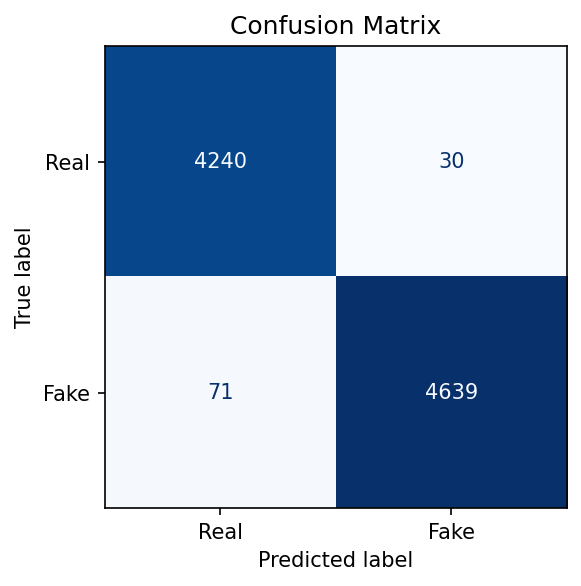
\includegraphics[width=0.5\textwidth]{../models/confusion_matrix.png}
\caption{Confusion matrix showing 4,240 true negatives, 4,639 true positives, 30 false positives, and 71 false negatives.}
\label{fig:cm}
\end{figure}

\textbf{Error Analysis:}
\begin{itemize}
    \item \textbf{False Positives (30):} Real articles misclassified as Fake — likely shorter articles lacking enough discriminative vocabulary.
    \item \textbf{False Negatives (71):} Fake articles misclassified as Real — likely well-written fabrications mimicking Reuters-style language.
\end{itemize}

% ============================================================
\section{Deployment}

\subsection{Streamlit Web Application}
The trained model is deployed as an interactive web application using Streamlit Community Cloud.

\begin{figure}[H]
\centering
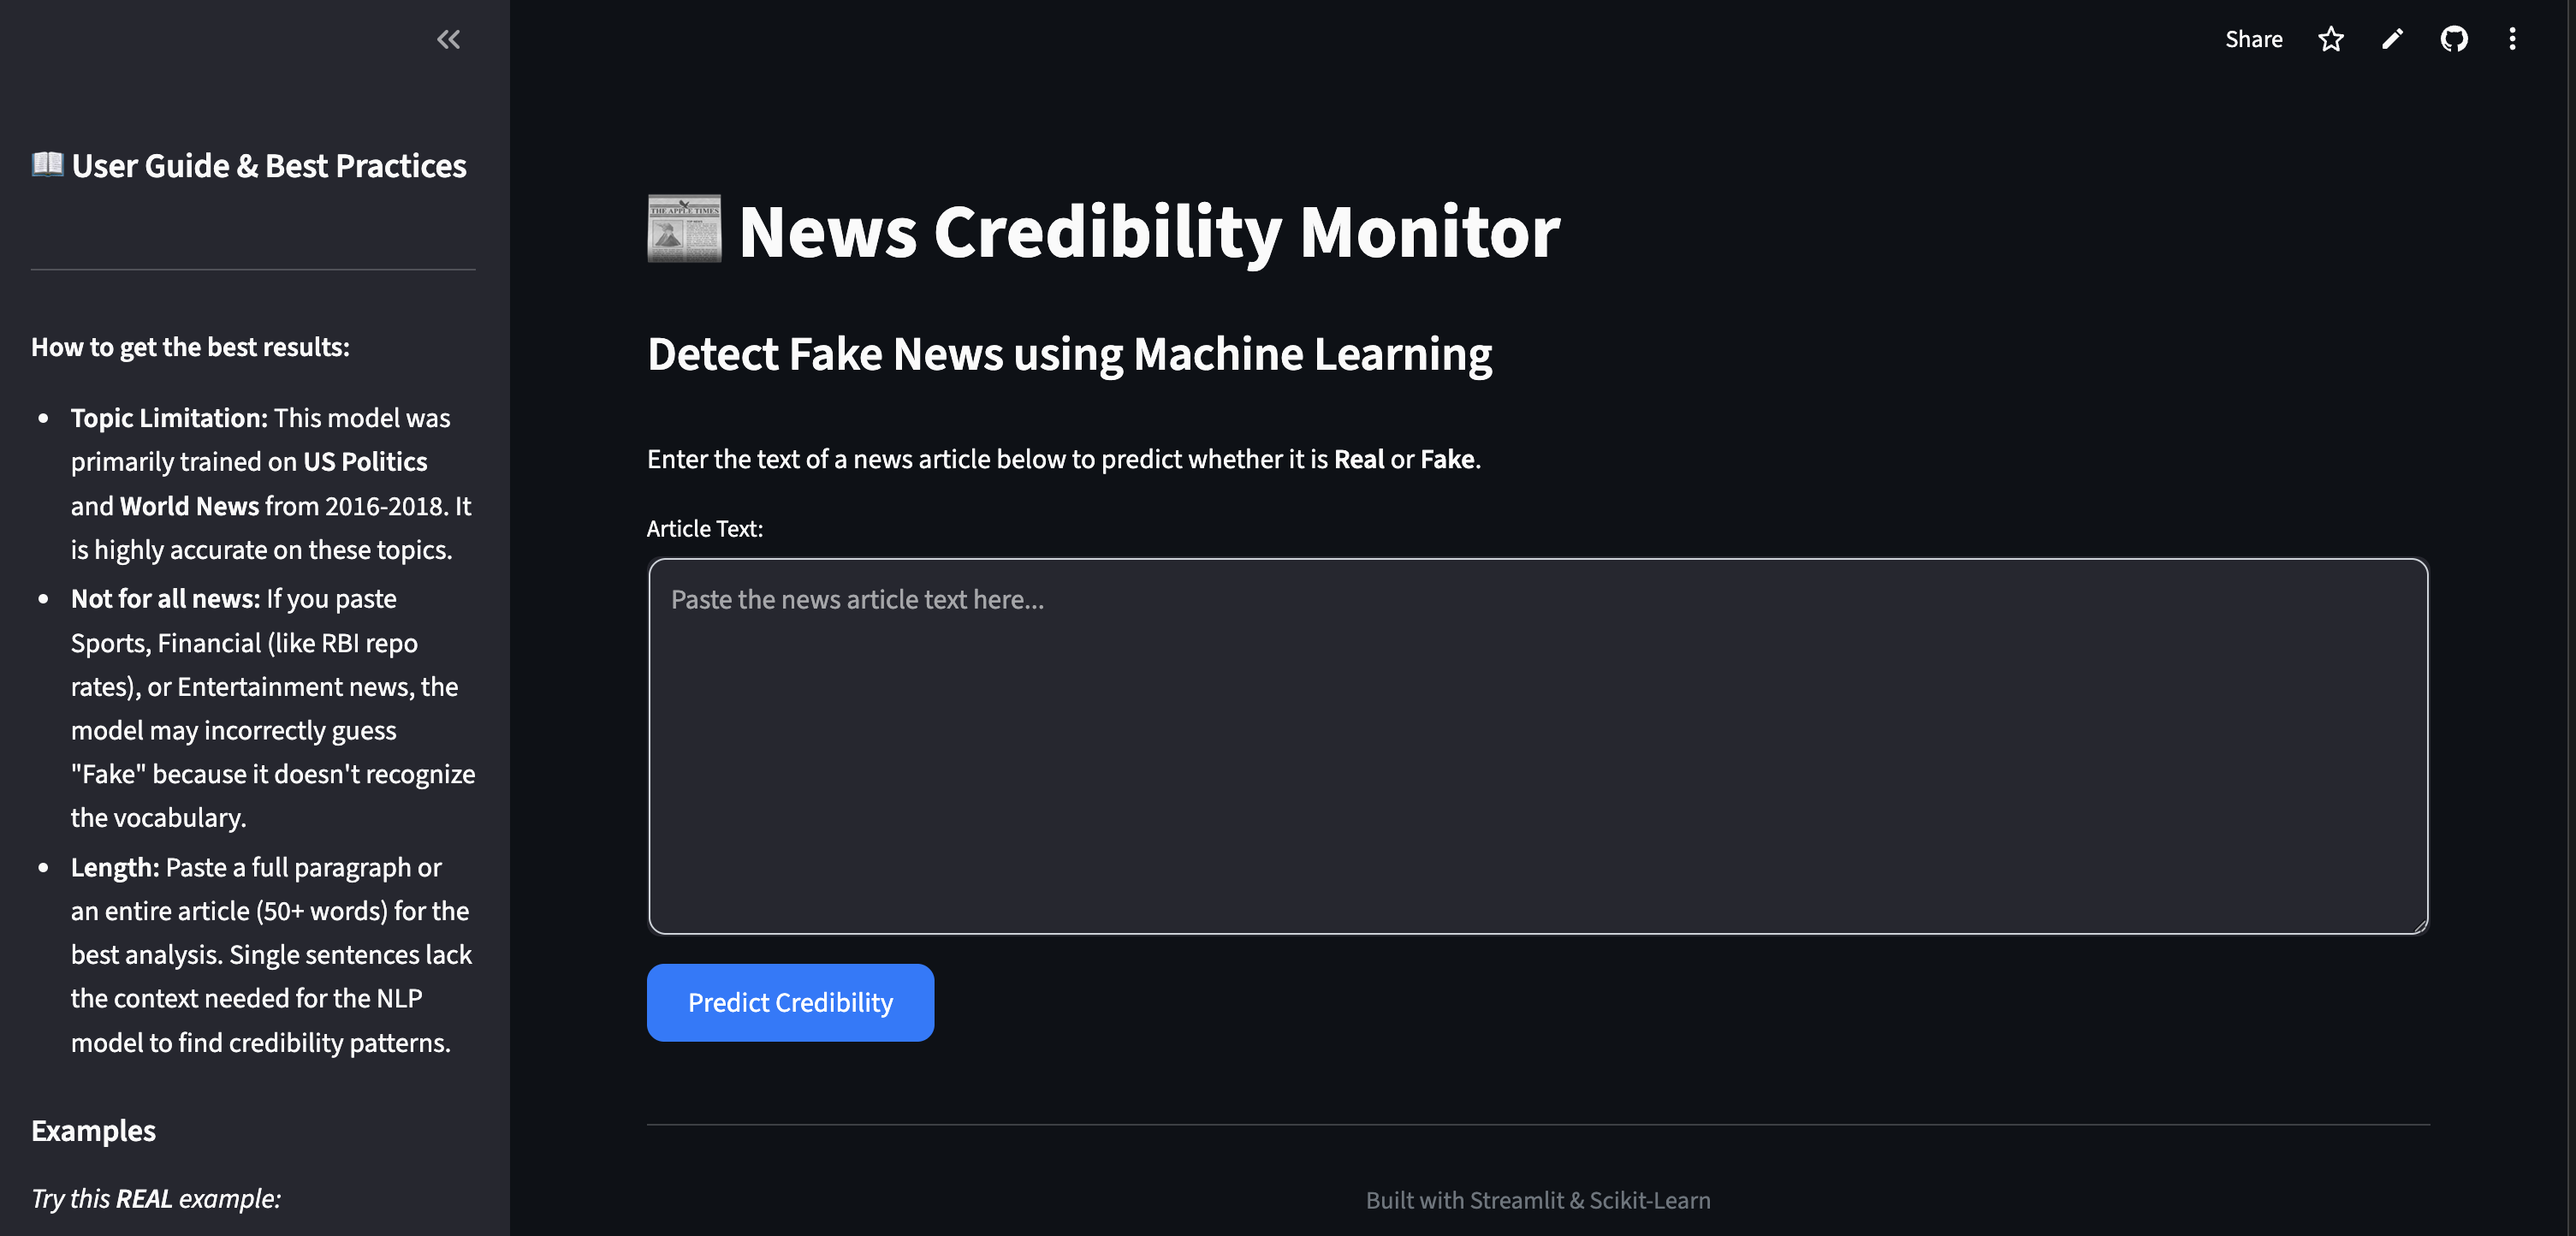
\includegraphics[width=0.75\textwidth]{../docs/ui.png}
\caption{Streamlit application interface showing the prediction result and confidence score.}
\label{fig:ui}
\end{figure}

\textbf{Key UX Features:}
\begin{itemize}
    \item \textbf{Input Validation:} Warns users when input text is too short ($<$20 meaningful words) for reliable classification.
    \item \textbf{Confidence Score:} Displays the model's predicted probability alongside the binary label.
    \item \textbf{User Guide Sidebar:} Educates users about the model's training domain and limitations.
    \item \textbf{Cached Model Loading:} Uses \texttt{@st.cache\_resource} for sub-second inference after cold start.
\end{itemize}

\subsection{Deployment Stack}
\begin{itemize}
    \item \textbf{Platform:} Streamlit Community Cloud
    \item \textbf{Requirements:} \texttt{requirements\_deploy.txt} (7 lean dependencies)
    \item \textbf{Model Artifacts:} \texttt{best\_model.pkl} (79 KB) and \texttt{tfidf\_vectorizer.pkl} (377 KB) via Git LFS
    \item \textbf{Live URL:} \url{https://news-credibility-monitor.streamlit.app/}
\end{itemize}

% ============================================================
\section{Code Quality \& Modularity}

The codebase follows a \textbf{Cookiecutter Data Science}-inspired structure:

\begin{table}[H]
\centering
\caption{Module Responsibilities}
\begin{tabular}{@{}llp{7cm}@{}}
\toprule
\textbf{Module} & \textbf{File} & \textbf{Responsibility} \\
\midrule
Config & \texttt{src/config/config.py} & Centralized path constants (no hardcoded paths elsewhere) \\
Data & \texttt{src/data/load\_data.py} & Load, label, merge, shuffle raw CSVs \\
Utils & \texttt{src/utils/text\_cleaner.py} & NLP preprocessing pipeline \\
Features & \texttt{src/features/build\_features.py} & TF-IDF vectorizer construction \\
Models & \texttt{src/models/train.py} & Model instantiation and fitting \\
Evaluation & \texttt{src/models/evaluate.py} & Metrics computation, JSON export, plots \\
Pipeline & \texttt{src/pipeline/training\_pipeline.py} & End-to-end orchestration \\
\bottomrule
\end{tabular}
\end{table}

\textbf{Design Principles:}
\begin{itemize}
    \item \textbf{Single Responsibility:} Each module performs exactly one task.
    \item \textbf{Reproducibility:} Fixed \texttt{random\_state=42}, serialized artifacts via Joblib.
    \item \textbf{Version Control:} Git LFS for large files; \texttt{.gitignore} for derived data.
\end{itemize}

% ============================================================
\section{Limitations \& Future Work}

\subsection{Current Limitations}
\begin{itemize}
    \item \textbf{Domain Specificity:} The model is trained exclusively on US political/world news (2016–2018) and may underperform on sports, finance, or entertainment articles.
    \item \textbf{Temporal Drift:} Language patterns in fake news evolve; the model may need retraining on contemporary data.
    \item \textbf{No Explainability Layer:} While Logistic Regression coefficients are interpretable, the app does not surface per-prediction explanations to users.
\end{itemize}

\subsection{Milestone 2 Roadmap}
\begin{itemize}
    \item Integration of LLM-based analysis for nuanced credibility assessment.
    \item Agentic AI workflows for multi-source fact verification.
    \item LIME/SHAP-based explainability in the Streamlit interface.
\end{itemize}

% ============================================================
\section{Conclusion}
This project demonstrates that a well-engineered traditional ML pipeline can achieve near-perfect accuracy (98.88\%) on the fake news detection task. The modular architecture, comprehensive evaluation, and production-grade Streamlit deployment satisfy all Milestone 1 requirements. The system provides a robust foundation for Milestone 2's integration of advanced AI techniques.

% ============================================================
\begin{thebibliography}{9}

\bibitem{ahmed2018detecting}
Ahmed, H., Traore, I., \& Saad, S. (2018).
\textit{Detecting opinion spams and fake news using text classification.}
Security and Privacy, 1(1), e9.

\bibitem{isot2020}
Ahmed, H., Traore, I., \& Saad, S. (2017).
\textit{Detection of Online Fake News Using N-Gram Analysis and Machine Learning Techniques.}
ISDDC 2017, LNCS, vol.\ 10618, pp.\ 127--138.

\bibitem{joachims1998text}
Joachims, T. (1998).
\textit{Text categorization with support vector machines: Learning with many relevant features.}
European Conference on Machine Learning, pp.\ 137--142.

\bibitem{sklearn}
Pedregosa, F.\ et al.\ (2011).
\textit{Scikit-learn: Machine Learning in Python.}
Journal of Machine Learning Research, 12, 2825--2830.

\end{thebibliography}

\end{document}
